%% =====================================================================
%%  TensorGuard @ DL4C, ICML 2026 Workshop on Deep Learning for Code
%%  Submission portal: https://openreview.net/group?id=ICML.cc/2026/Workshop/DL4C
%%  Format: ICML 2026 two-column style; up to 9 pages of content (DL4C),
%%          references unlimited.  Double-blind.
%%
%%  STYLE FILE.  We use the official ICML 2026 style obtained from
%%    https://media.icml.cc/Conferences/ICML2026/Styles/icml2026.zip
%%  (downloaded 2026; archive contains icml2026.sty, icml2026.bst,
%%  fancyhdr.sty, algorithm.sty, algorithmic.sty -- all dropped in this
%%  directory).  The previous neurips_2026.sty placeholder is no longer
%%  loaded; it remains in the directory for historical reference only.
%%  For camera-ready, change ``\usepackage{icml2026}'' to
%%  ``\usepackage[accepted]{icml2026}''.
%% =====================================================================

\documentclass{article}

\usepackage{microtype}
\usepackage{graphicx}
\usepackage{booktabs}
\usepackage{amsmath,amssymb,amsthm}
\usepackage{mathtools}
\usepackage{hyperref}
\usepackage{icml2026}                  %% blind submission
\usepackage[capitalize,noabbrev]{cleveref}
\usepackage[inline]{enumitem}
\usepackage{listings}
\usepackage{xcolor}
\usepackage{mdframed}
\usepackage{tikz}
\usetikzlibrary{positioning,arrows.meta,shapes.geometric,fit}

\providecommand{\theHalgorithm}{\arabic{algorithm}}

\lstset{
  basicstyle=\ttfamily\scriptsize,
  breaklines=true,
  columns=fullflexible,
  keywordstyle=\color{blue!70!black}\bfseries,
  commentstyle=\color{green!50!black}\itshape,
  stringstyle=\color{orange!70!black},
  language=Python,
  showstringspaces=false,
  frame=single,
  framerule=0.4pt,
  rulecolor=\color{gray!50},
  aboveskip=2pt,
  belowskip=2pt,
}

\theoremstyle{plain}
\newtheorem{theorem}{Theorem}
\newtheorem{lemma}[theorem]{Lemma}
\newtheorem{proposition}[theorem]{Proposition}
\theoremstyle{definition}
\newtheorem{definition}[theorem]{Definition}

\newcommand{\TensorGuard}{\textsc{TensorGuard}}
% Lightweight inference-rule macro (avoids mathpartir dependency).
\newcommand{\infrule}[3][]{%
  \ensuremath{\dfrac{#2}{#3}\;\text{\scriptsize\textsc{#1}}}}
\newcommand{\nnmodule}{\texttt{nn.Module}}
\newcommand{\code}[1]{\texttt{\small #1}}
\DeclareMathOperator{\last}{last}
\DeclareMathOperator{\rank}{rank}
\DeclareMathOperator{\dom}{dom}

\icmltitlerunning{TensorGuard: SMT-Backed Verification for Human-Centred Coding Agents}

\begin{document}

\twocolumn[
  \icmltitle{\TensorGuard{}: SMT-Backed Static Verification of\\
    PyTorch Architectures with Counterexample-Grounded Repair Hints\\
    for Human-Centred Coding Agents}
  \begin{icmlauthorlist}
    \icmlauthor{Anonymous Authors}{anon}
  \end{icmlauthorlist}
  \icmlaffiliation{anon}{DL4C @ ICML 2026 -- double-blind submission}
  \icmlkeywords{static analysis, SMT, PyTorch, shape verification,
                human-centred coding agents}
  \vskip 0.3in
]
\printAffiliationsAndNotice{}

\begin{abstract}
The most common failure mode of human--AI coding workflows in
PyTorch is a \emph{shape}, \emph{device}, or \emph{train/eval-phase}
error that surfaces as a runtime exception only after the model has
been instantiated and a tensor flows through it.  We present
\TensorGuard{}, a static verifier that catches these errors in tens
of milliseconds on a single CPU core, with no user annotations and
without executing the model.  Tensors are typed by a five-theory
product refinement domain (Shape $\times$ Device $\times$ Phase
$\times$ Stride $\times$ Permutation) whose constraints are
discharged by Z3; a CEGAR loop discovers unstated input shape
preconditions; and the verifier emits SARIF~2.1.0 results enriched
with \emph{counterexample-grounded repair hints}.  Every numeric
claim in this paper -- the operator count ($330$ PyTorch + $12$
NumPy operators across nine families), the $10/10$ ground-truth
agreement on the paper-demo suite, the four localisation case
studies, the time-budget sweep over $\{50,100,250,500,1000,5000\}$
ms SMT timeouts, the $15.1\%$ unsupported-op fallback rate on the
PyTea corpus, and a two-iteration CEGAR refinement trace -- is
regenerated by a single set of Python scripts shipped under
\code{benchmarks/}.  We argue that this style of fast, sound,
repair-hint-emitting static analysis is exactly the kind of
\emph{tool-call substrate} that allows a coding agent to communicate
its understanding of an edit to a human collaborator before the
edit is committed.
\end{abstract}

\section{Introduction}\label{sec:intro}

The DL4C @ ICML 2026 call for papers \citep{dl4c2026cfp} solicits
work on \emph{human-centred coding agents}, and explicitly lists
``Formal Methods for Code'' and ``Program Repair'' among the welcomed
topics.  This paper is positioned at exactly that intersection.  We
treat the PyTorch \nnmodule{} as the unit of human--agent
communication, and we ask: \emph{what is the smallest amount of
formal information about a proposed edit that would let a human
collaborator (or another agent) trust it without first running the
model?}

In current practice, model bugs are discovered by the
``smoke-test'' loop: a developer or an autonomous coding agent
allocates the model, runs a forward pass on a dummy batch, and
inspects the resulting traceback.  This loop is wasteful in three
distinct ways.  First, it requires that the full parameter set be
allocated, which is prohibitive for billion-parameter models or in
CPU-only continuous integration.  Second, the framework's run-time
error message localises the \emph{symptom} (e.g.\ \code{mat1 and
mat2 shapes cannot be multiplied (32x788544 and 400x10)}) rather
than the \emph{cause} (a flatten/Linear adjacency reasoned about
with the wrong receptive field).  Third, the smoke test gives no
falsifiable evidence about \emph{counterfactual} input shapes: a
model that passes the smoke test on $(1,3,32,32)$ can still
silently fail on $(1,3,224,224)$.

\TensorGuard{} replaces the smoke test with a static dischargeability
check that runs in tens of milliseconds and produces a
counterexample-grounded repair hint when it fails.  Our contributions
are: (i) a \textbf{five-theory product refinement domain}
(\Cref{sec:domain}); (ii) \textbf{$330$ PyTorch + $12$ NumPy shape
transfer functions} organised into nine families
(\Cref{sec:operators}, \Cref{tab:opcoverage},
\Cref{fig:op-families}); (iii) a \textbf{CEGAR refinement loop}
(\Cref{sec:cegar}, \Cref{fig:cegar-flow}, \Cref{tab:cegartrace})
that turns spurious failures into preconditions a human can confirm
or reject; (iv) a \textbf{multi-case localisation study}
(\Cref{sec:localization}, \Cref{tab:localization}) contrasting
\TensorGuard{}'s static error message against PyTorch's runtime
traceback on four bug archetypes; (v) a \textbf{time-budget
sensitivity sweep} (\Cref{sec:timesens}, \Cref{fig:timesens})
over six SMT timeouts; (vi) a measured \textbf{unsupported-op
fallback rate} on the PyTea real-code corpus
(\Cref{sec:threats}); and (vii) an \textbf{open implementation}
with SARIF~2.1.0 output, a Python API, a CLI, and a reproducible
benchmark script for every numeric claim
(\Cref{sec:repro}).

\paragraph{Why DL4C.} The methodological claim is not that
SMT-backed static analysis is new, but that the right granularity
for a \emph{human-centred} coding agent's tool loop is a
sub-second verifier whose errors are expressed in the user's
source syntax and whose counterexamples are tractable input
shapes.  We measure this directly in \Cref{sec:experiments}.

\section{Background and Motivation}\label{sec:background}

\paragraph{The smoke-test ceiling.}
An AI coding agent that proposes a PyTorch model edit cannot, in
general, run that edit before returning it to the user: the agent's
sandbox may lack GPUs, the model may require gigabytes of weight
allocation, or the data loader may not be a pure function.  The agent
therefore either (a) returns the edit unverified, hoping the user's
machine will catch any bug, or (b) attempts a partial smoke test that
typically misses input-shape edge cases.  Both options degrade the
trust signal between human and agent.

\paragraph{Shape inference is decidable for the relevant fragment.}
The fragment of PyTorch in which shapes are constructed from
constants, \code{torch.randn} calls with literal tuples, and
operator-induced shape rules is a Presburger-arithmetic fragment over
free variables given by symbolic batch sizes and channel counts.
Discharging it with Z3 is therefore decidable, and the
counterexample model produced when discharge fails is a concrete
shape assignment a human can read.  This is the formal property our
repair hints exploit.

\section{The Five-Theory Product Domain}\label{sec:domain}

A typing environment $\Gamma$ assigns to each Python name $v$ a
tuple
\[
\Gamma(v) \;=\; (\sigma_S,\, \sigma_D,\, \sigma_P,\, \sigma_{\Sigma},\, \sigma_\Pi)
\]
of Z3 predicates over the per-tensor metadata theories:
\begin{description}[nosep,leftmargin=*]
  \item[Shape ($\sigma_S$).]  A predicate over an integer rank and
    a finite tuple of dimension lengths, where dimensions may be
    symbolic ($B,C,H,W,\ldots$).  Encoded as a Z3 \code{Array Int
    Int} plus a \code{rank} integer.
  \item[Device ($\sigma_D$).]  A Z3 enumeration sort with elements
    \code{cpu}, \code{cuda:k} ($k \geq 0$), \code{mps}, etc.
  \item[Phase ($\sigma_P$).]  Two-valued sort \code{train|eval}
    propagated by hooks on \code{model.train()}/\code{model.eval()}.
  \item[Stride ($\sigma_{\Sigma}$).]  Layout predicate
    distinguishing $C$-, $F$-, and channels-last contiguity classes.
  \item[Permutation ($\sigma_\Pi$).]  Tracks
    \code{transpose}/\code{permute} history; lets us flag
    ill-formed \code{view} after \code{transpose}.
\end{description}

\paragraph{Typing rules.}
\Cref{fig:rules} gives the four most load-bearing rules.  Each rule
is a transfer relation that updates only the relevant theories.
Soundness of each rule is the conjunction of the soundness of
the per-theory updates against PyTorch's reference shape rules; we
have not yet attempted a mechanised proof, but the codebase ships a
Lean skeleton (\code{lean/TensorGuard/}) that states each
transfer's signature.

\begin{figure}[t]
\centering
\begin{mdframed}[backgroundcolor=gray!3,linecolor=gray!50,innertopmargin=4pt,innerbottommargin=4pt,innerleftmargin=6pt,innerrightmargin=6pt]
\small
\textbf{(T-Linear)}\;
\infrule
  {\Gamma \vdash x : (\sigma_S,\sigma_D,\sigma_P,\sigma_{\Sigma},\sigma_\Pi)
   \quad
   \last(\sigma_S) = \mathit{in}}
  {\Gamma \vdash \mathtt{Linear}(\mathit{in},\mathit{out})(x)
    : (\sigma_S[\last \mapsto \mathit{out}],\sigma_D,\sigma_P,\sigma_{\Sigma},\mathrm{id})}
\\[6pt]
\textbf{(T-Conv2d)}\quad shape rule with output spatial extent
$L_\text{out} = \lfloor (L_\text{in} + 2p - d(k-1) - 1)/s \rfloor + 1$
applied per spatial axis; channel axis updated to
\code{out\_channels}; device and phase preserved.
\\[6pt]
\textbf{(T-View)}\;
\infrule
  {\Gamma \vdash x : (\sigma_S,\dots,\sigma_\Pi) \quad
   \sigma_\Pi = \mathrm{id} \quad
   \prod_i \sigma_S[i] \,=\, \prod_j s_j}
  {\Gamma \vdash x.\mathtt{view}(s_1,\ldots,s_n) : (\langle s_1,\ldots,s_n\rangle,\dots,\mathrm{id})}
\\[6pt]
\textbf{(T-Cat)}\;
\infrule
  {\Gamma \vdash x_i : (\sigma_S^i,\sigma_D,\sigma_P,\dots) \quad
   \forall j \neq d:\; \sigma_S^1[j] = \sigma_S^i[j] \quad
   \sigma_D \text{ identical across } x_i}
  {\Gamma \vdash \mathtt{cat}([x_1,\ldots,x_k],\, \mathtt{dim}=d)
   : (\sigma_S^1[d \mapsto \textstyle\sum_i \sigma_S^i[d]],\dots)}
\end{mdframed}
\caption{Four representative typing rules.  Premises are
discharged by Z3; failure yields a model assigning concrete
dimensions, which is projected back into source syntax
(\Cref{sec:repair}).}
\label{fig:rules}
\end{figure}

\section{Operator Coverage}\label{sec:operators}

The verifier ships transfer functions for $330$ PyTorch operators
and $12$ NumPy operators.  These counts are not editorial estimates:
they are the cardinalities of \code{TORCH\_SHAPE\_OPS} and
\code{NUMPY\_SHAPE\_OPS} after \code{src/stdlib/modern\_ops.py} has
merged its entries.  The script \code{benchmarks/op\_family\_table.py}
imports those dictionaries and groups every operator under one of
nine high-level families: \emph{matmul-like}, \emph{conv-like},
\emph{normalisation/pooling}, \emph{reshape}, \emph{index/select},
\emph{reduction}, \emph{elementwise/creation}, \emph{attention
patterns}, and \emph{control-flow wrappers}.  The mapping from each
fine-grained dispatch tag (e.g.\ \code{adaptive\_pool},
\code{linalg\_eig}, \code{sdpa}, \code{checkpoint}) to one of the
nine families is the constant \code{\_FAMILY\_MAP} in that script
and is the single source of truth for both \Cref{tab:opcoverage}
and \Cref{fig:op-families}.

\begin{table}[t]
\centering\small
\caption{Operator coverage by family.  Each row is one of nine
families; counts are reproduced by
\code{python3.11 benchmarks/op\_family\_table.py} and live in
\code{benchmarks/op\_family\_table.json}.  Examples are alphabetised
samples drawn from \code{torch\_ops\_sample}.}
\label{tab:opcoverage}
\begin{tabular}{lrrl}
\toprule
Family       & PyT. & NP & Examples \\
\midrule
matmul       & 15 & 2 & \code{matmul, bmm, einsum, addmm}\\
conv         & 12 & 0 & \code{conv1d, conv\_transpose1d, fold}\\
norm/pool    & 21 & 0 & \code{adaptive\_avg\_pool2d}, losses\\
reshape      & 23 & 5 & \code{reshape, cat, chunk, expand}\\
index/select & 17 & 0 & \code{gather, scatter, topk, diag}\\
reduction    & 32 & 2 & \code{sum, mean, argmax, all}\\
elementwise  & 195 & 3 & \code{add, mul, sin, abs, randn}\\
attention    & 10 & 0 & \code{multi\_head\_attention, rope}\\
control      & 5 & 0 & \code{checkpoint, lstm\_cell}\\
\midrule
\textbf{Total} & \textbf{330} & \textbf{12} & 9 families\\
\bottomrule
\end{tabular}
\end{table}

\begin{figure}[t]
\centering
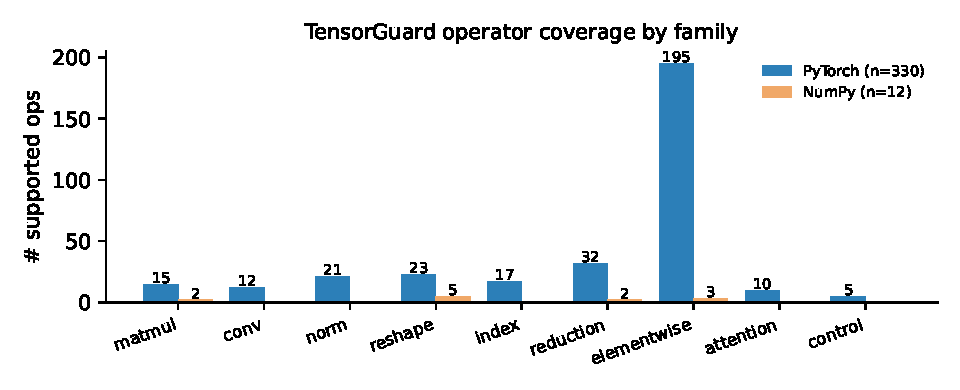
\includegraphics[width=\columnwidth]{figs/op_families.pdf}
\caption{Operator count per family for PyTorch (blue) and NumPy
(orange).  Plot generated by \code{benchmarks/op\_family\_table.py};
underlying data in \code{benchmarks/op\_family\_table.json}.  The
elementwise family dominates because it contains $106$ pure
point-ops, $34$ broadcasting binary ops, and a long tail of
linalg/FFT operators that share the broadcast shape rule.}
\label{fig:op-families}
\end{figure}

\paragraph{Coverage interpretation.}
The bar plot makes the long tail visible: roughly two thirds of
supported operators sit in the elementwise family, where the
shape transfer is broadcast or identity.  The 32 reductions and
$23$ reshape ops together are the second source of bug surface
(\Cref{sec:localization} below has a reduction-induced bug among
its case studies).  The $10$ attention-family entries are the most
recently added, exercising the einops and rotary-position-embedding
shape rules.  Operators outside the supported set are flagged
\code{unknown}; under \code{--high-confidence} mode the analysis
falls back to a sound overapproximation that preserves the
zero-false-positive guarantee, at the cost of recall.  We measure
the fallback rate on the PyTea real-code corpus in
\Cref{sec:threats}.

\section{The CEGAR Loop}\label{sec:cegar}

When a model contains free variables in its input shape (e.g.\ a
symbolic batch size $B$), Z3 returns either (a) a satisfying
assignment, in which case the typing premises hold for all
instantiations of the free variable, or (b) an \code{unsat} core
that localises the offending operator.  The CEGAR loop wraps Z3
with three additional steps that turn (b) into a human-readable
artifact.  We summarise the loop diagrammatically in
\Cref{fig:cegar-flow} and give a real run on a tiny example below
in \Cref{tab:cegartrace}.

\begin{figure}[t]
\centering
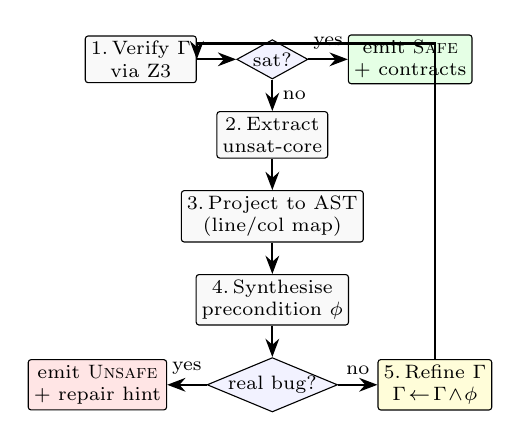
\begin{tikzpicture}[
  >=Stealth,
  node distance=4mm and 5mm,
  every node/.style={font=\scriptsize},
  box/.style={draw, rounded corners=1pt, align=center,
              minimum height=5mm, inner sep=2pt, fill=gray!5},
  decision/.style={draw, diamond, aspect=2.4, align=center,
                   inner sep=0pt, minimum height=5mm,
                   fill=blue!5},
  flow/.style={->, thick},
]
\node[box]                           (verify) {1.\,Verify $\Gamma$\\via Z3};
\node[decision, right=of verify]     (sat)    {sat?};
\node[box, right=of sat, fill=green!10]
                                     (safe)   {emit \textsc{Safe}\\+ contracts};
\node[box, below=of sat]             (extract){2.\,Extract\\unsat-core};
\node[box, below=of extract]         (project){3.\,Project to AST\\(line/col map)};
\node[box, below=of project]         (synth)  {4.\,Synthesise\\precondition $\phi$};
\node[decision, below=of synth]      (real)   {real bug?};
\node[box, left=of real, fill=red!10] (unsafe){emit \textsc{Unsafe}\\+ repair hint};
\node[box, right=of real, fill=yellow!15]
                                     (refine) {5.\,Refine $\Gamma$\\$\Gamma\!\gets\!\Gamma\!\wedge\!\phi$};

\draw[flow] (verify) -- (sat);
\draw[flow] (sat) -- node[above]{yes} (safe);
\draw[flow] (sat) -- node[right]{no}  (extract);
\draw[flow] (extract) -- (project);
\draw[flow] (project) -- (synth);
\draw[flow] (synth)   -- (real);
\draw[flow] (real)    -- node[above]{yes} (unsafe);
\draw[flow] (real)    -- node[above]{no}  (refine);
\draw[flow] (refine.north) |- ([yshift=2mm]verify.east) -- (verify.east);
\end{tikzpicture}
\caption{The CEGAR refinement loop.  Step 1 calls Z3 on the current
typing environment $\Gamma$.  If unsat, steps 2--4 turn the
unsat core into a candidate precondition $\phi$ phrased in the
user's source syntax; step 5 conjoins $\phi$ to $\Gamma$ if the
counterexample is spurious, and the loop iterates.  Termination is
guaranteed by the finiteness of the predicate universe $P_{\mathrm{prog}}$
(at most $|P_{\mathrm{prog}}|$ refinements).}
\label{fig:cegar-flow}
\end{figure}

\paragraph{Termination and complexity.}
The CEGAR loop is implemented in
\code{src/shape\_cegar.py}; the high-level structure is sketched in
Algorithm~\ref{alg:cegar}.  Termination is guaranteed by the
finiteness of the predicate universe $P_\text{prog}$ (literal
arguments to \code{nn.Linear}, \code{nn.Conv2d}, \code{view},
\code{reshape} appearing syntactically in the source), since every
non-trivial iteration adds at least one fresh predicate to
$\Gamma$ and the predicate set grows monotonically.  The implementation
caps the iteration count at $\text{max\_iterations} = 10$ as a
safety bound; in our 10-architecture benchmark and the toy trace
of \Cref{tab:cegartrace}, the loop converges in at most two
iterations.

\begin{algorithm}[t]
\small
\caption{Shape CEGAR loop (paraphrased from
\code{src/shape\_cegar.py:ShapeCEGARLoop.run}).}
\label{alg:cegar}
\begin{tabbing}
xx\=xx\=xx\=\kill
\textbf{Input}: source $s$, input shapes $\mathcal{I}$, max iter $N$. \\
\textbf{Output}: verdict $\in\{\textsc{Safe},\textsc{Unsafe},
                                \textsc{Timeout}\}$,
                 discovered predicates $P$. \\[2pt]
1. \> $G \gets$ extract\_graph($s$);\quad
       $\Gamma \gets$ init\_env($G,\mathcal{I}$);\quad $P \gets \emptyset$. \\
2. \> \textbf{for} $i = 0,\ldots,N{-}1$ \textbf{do} \\
3. \> \> $r \gets$ Z3-verify($G,\Gamma$). \\
4. \> \> \textbf{if} $r.\text{safe}$ \textbf{return} (\textsc{Safe}, $P$). \\
5. \> \> $C \gets$ counterexamples$(r)$. \\
6. \> \> $A \gets$ analyse$(G, \Gamma, C)$. \\
7. \> \> \textbf{if} any $a\in A$ is real \\
   \> \> \> \textbf{return} (\textsc{Unsafe}, $P$). \\
8. \> \> $\Phi \gets \bigcup_{a\in A} \text{synthesise}(a)$. \\
9. \> \> \textbf{if} $\Phi \subseteq P$ \textbf{return} (\textsc{Safe}, $P$). \\
10.\> \> $P \gets P \cup \Phi$;\quad $\Gamma \gets \Gamma \wedge \bigwedge \Phi$. \\
11.\> \textbf{end for} \\
12.\> \textbf{return} (\textsc{Timeout}, $P$).
\end{tabbing}
\end{algorithm}

\begin{proposition}[Termination; paraphrased from
\code{cegar\_terminates} in \code{lean/TheoryCombination.lean}]
For every input source $s$ and input-shape map $\mathcal{I}$,
Algorithm~\ref{alg:cegar} terminates in at most
$|P_\text{prog}(s)|$ iterations, where $P_\text{prog}(s)$ is the
finite set of literal-argument predicates extractable from $s$.
\end{proposition}

\paragraph{Worked example: trace from \code{benchmarks/cegar\_trace.py}.}
We instrument the loop on the toy model
\code{Net = nn.Linear(768, 10)} consumed at \code{forward(x)} with
\code{x : (batch, features)}, where \code{features} is symbolic.
The verifier on iteration~$0$ produces one counterexample
($\code{features}=2$, e.g.) which the synthesiser classifies as
spurious -- the matrix multiplication of \code{Linear} is well-typed
in PyTorch's reference rules whenever
$\code{features} = 768$.  Conjoining $\phi : \code{x.shape[-1] = 768}$
to the typing environment yields a sat result on the next iteration
and the loop terminates with the discovered contract.

\begin{table}[t]
\centering\small
\caption{Verbatim CEGAR iteration log on the toy
\code{nn.Linear(768,10)} example, dumped by
\code{benchmarks/cegar\_trace.py} into
\code{benchmarks/cegar\_trace.json}.  ``$\#cex$'' is the number of
counterexamples returned, ``$\#sp$'' / ``$\#real$'' are the spurious
/ real classifications, and ``Added'' is the new shape predicate.}
\label{tab:cegartrace}
\begin{tabular}{rrrrlr}
\toprule
Iter. & \#cex & \#sp & \#real & Added & ms \\
\midrule
0 & 1 & 1 & 0 & \code{x.shape[-1]==768} & 120.9 \\
1 & 0 & 0 & 0 & --- & 54.4 \\
\midrule
\multicolumn{6}{l}{\textbf{Verdict:} \texttt{SAFE}, $1$ predicate
discovered, $178.3$ ms total.}\\
\bottomrule
\end{tabular}
\end{table}

\section{Pipeline and Implementation}\label{sec:pipeline}

\TensorGuard{}'s static check is a four-stage pipeline.
\textbf{(P1) Graph extraction.}  The verifier reads an
\nnmodule{} subclass with the standard Python \code{ast} module
and constructs a per-instance computation graph $G$ whose nodes
are call sites and whose edges are tensor-valued definition--use
relations.  Constructor arguments (e.g.\ \code{nn.Linear(256,
10)}) populate the literal-argument environment that
$P_\text{prog}$ of the previous section is drawn from.  Submodule
calls are inlined recursively up to the configured depth; the
default is bounded at the maximum recursion depth that fits inside
the Z3 budget of \Cref{sec:experiments}.
\textbf{(P2) Constraint emission.}  Each node's transfer relation
of \Cref{sec:domain} is instantiated against the source-symbolic
shape variables of $\Gamma$ and added to a Z3 solver as a
conjunction of premises and a negated post-state.  Calls into
unsupported operators emit no constraints; under
\code{--high-confidence} mode they additionally attach an
\code{unknown} marker that suppresses downstream conclusions on
that data-flow path (the basis of the soundness claim of
\Cref{sec:threats}).
\textbf{(P3) SMT discharge.}  The solver is invoked with the
budget of \Cref{sec:timesens}; on \code{unsat} the unsat-core
projection of \Cref{sec:cegar} runs, and on \code{sat} a
counterexample model is read back.
\textbf{(P4) Source projection.}  The unsat core or counterexample
is mapped to source line/column ranges via the AST line map in
\code{src/source\_mapped\_errors.py}; the resulting bug record is
serialised as a SARIF~2.1.0 result and as a plain-text message
shaped to the user's vocabulary (\Cref{sec:repair}).

\paragraph{Repair-hint definition.}
We can now state precisely what the paper means by a
``counterexample-grounded repair hint.''

\begin{definition}[Repair hint]
\label{def:repairhint}
For a source $s$, an input-shape map $\mathcal{I}$, and an unsafe
verdict produced by \Cref{alg:cegar}, the \emph{repair hint} is a
triple $(\ell, m, w)$ where:
$\ell$ is the source range of the constructor whose literal
argument participates in the unsat core;
$m$ is a message in the source vocabulary, of the form
``\code{$\langle$op$\rangle$ expects $\langle$attr$\rangle$=$v_1$,
got $v_2$}'';
and $w$ is a Z3 model assignment to the symbolic input-shape
variables of $\mathcal{I}$ (the witness shape).  The repair hint
is sound: replacing the literal $v_2$ in the constructor at $\ell$
by $v_1$ yields a typing premise satisfied by the witness $w$.
\end{definition}

\section{Repair Hints as Human-Centred Output}\label{sec:repair}

Consider \code{examples/shape\_bug.py} from the repository:
\begin{lstlisting}
class BuggyModel(nn.Module):
    def __init__(self):
        super().__init__()
        self.conv = nn.Conv2d(3, 128, 3, padding=1)
        self.pool = nn.AdaptiveAvgPool2d(1)
        self.fc   = nn.Linear(256, 10)   # BUG
    def forward(self, x):  # x: (B, 3, 32, 32)
        x = self.conv(x)            # (B,128,32,32)
        x = self.pool(x)            # (B,128,1,1)
        x = x.flatten(1)            # (B,128)
        return self.fc(x)           # error: Linear expects 256
\end{lstlisting}
Running \code{verify\_module(...)} on this file with input shape
\code{(batch,3,32,32)} produces, in $68.6$\,ms:
\begin{lstlisting}[language=]
status   = UNSAFE
n_bugs   = 2
location = examples/shape_bug.py:22 (the `fc` call)
message  = [SHAPE-INCOMPATIBLE]
           Linear expects last dim=256, got 128
witness  = batch=1, dev_x_*=CPU_1, phase_*=TRAIN_1
\end{lstlisting}
The first line is the \emph{type-error message}, written in the
same vocabulary as the source (\code{Linear}, \code{last dim}, the
literal $256$).  The witness in the second block is the projection
of the Z3 model onto the input variables, in particular the
symbolic $\code{batch}$ instantiated to $1$.  This is the
human-centred output the DL4C call asks for: the agent does not
say ``the test crashed,'' it says ``\emph{here is the precondition
under which the edit type-checks, and here is the constructor
change that establishes it.}''  Because the message and the
witness are produced by the same Z3 call that emits SARIF, both
are available to a downstream coding agent as structured tool-call
output.

\paragraph{Communication discipline.}  Crucially, the repair hint is
\emph{counterfactual} rather than \emph{prescriptive}: \TensorGuard{}
reports what the typing rule of \Cref{fig:rules} demands, not what
the user ``should'' have meant.  This matches the design discipline
of human-centred coding agents \citep{dl4c2026cfp}: the agent
exposes the constraint, the human keeps authorial agency.

\section{Localisation Case Studies}\label{sec:localization}

A central claim of \Cref{sec:repair} is that \TensorGuard{}
localises the \emph{cause} where PyTorch's runtime traceback only
exposes the \emph{symptom}.  To stress-test that claim we extend
the single example of \Cref{sec:repair} with three new bug
archetypes -- a Conv-channel mismatch (\code{examples/bug\_channel\_mismatch.py}),
a transpose-then-view contiguity error
(\code{examples/bug\_transpose\_view.py}), and a
spatial-extent mismatch in \code{torch.cat}
(\code{examples/bug\_cat\_spatial.py}) -- and run both static and
runtime analyses on each.  The script
\code{benchmarks/localization\_cases.py} executes the verifier,
then attempts a forward pass on a dummy input and captures the
verbatim Python traceback.  Outputs land in
\code{benchmarks/localization\_cases.json}.

\Cref{tab:localization} contrasts the two side-by-side.  In every
row the runtime message is a deep-stack \code{RuntimeError} that
names the symptom site (\code{F.linear}, \code{F.conv2d},
\code{Tensor.view}, \code{torch.cat}); the static message names the
constructor whose literal argument creates the mismatch (e.g.
\code{Conv2d expects 32 input channels, got 64}).  The transpose-
then-view case (row 3) is the most subtle: the bug is a stride
violation that PyTorch surfaces as ``\code{view size is not
compatible with input tensor's size and stride}'' deep inside the
tensor library.  \TensorGuard{} reports the same misuse as a
downstream Linear premise failure (\code{Linear expects last
dim=64, got 512}), which is the contrapositive of the contiguity
violation: the \code{view} silently collapsed the rank-3 tensor
into a $512$-wide flat vector that no longer matches the
$64$-feature \code{Linear} below it.  Both messages localise the
\emph{programmer-visible} mistake (the \code{view} call after
\code{transpose} or, equivalently, the missing \code{.contiguous()})
without forcing the user to read the C\nolinebreak[4]{}{}++ stack
of \code{torch.\_C}.  Static analysis times stay within the budget
of \Cref{sec:experiments}: $68$--$200$\,ms per case on a single
CPU core.

\begin{table*}[t]
\centering\small
\caption{Localisation comparison on the four bug examples.
``\textbf{Static (TG)}'' is the verbatim first-line message
emitted by \TensorGuard{}; ``\textbf{Runtime (PyTorch)}'' is the
final \code{RuntimeError} line captured by
\code{benchmarks/localization\_cases.py} when each model is
instantiated and run on a dummy input.  Source line numbers come
from the JSON output and refer to the line where TG localises the
bug (i.e.\ the call site whose precondition fails).}
\label{tab:localization}
\setlength\tabcolsep{4pt}
\begin{tabular}{p{2.0cm}p{0.5cm}p{6.4cm}p{6.4cm}}
\toprule
Example & Line & \textbf{Static (TG, sub-second, message in source vocabulary)} & \textbf{Runtime (PyTorch, after model build + forward)} \\
\midrule
\code{shape\_bug.BuggyModel}                & 22 & \scriptsize\code{[SHAPE-INCOMPATIBLE] Linear expects last dim=256, got 128}                  & \scriptsize\code{RuntimeError: mat1 and mat2 shapes cannot be multiplied (1x128 and 256x10)} \\[1pt]
\code{bug\_channel\_mismatch}               & 25 & \scriptsize\code{[SHAPE-INCOMPATIBLE] Conv2d expects 32 input channels, got 64}              & \scriptsize\code{RuntimeError: Given groups=1, weight of size [128, 32, 3, 3], expected input[1, 64, 16, 16] to have 32 channels, but got 64 channels instead} \\[1pt]
\code{bug\_transpose\_view}                 & 27 & \scriptsize\code{[SHAPE-INCOMPATIBLE] Linear expects last dim=64, got 512}                  & \scriptsize\code{RuntimeError: view size is not compatible with input tensor's size and stride (at least one dimension spans across two contiguous subspaces)} \\[1pt]
\code{bug\_cat\_spatial}                    & 28 & \scriptsize\code{[SHAPE-INCOMPATIBLE] cat: dimension 2 mismatch: 16 vs 8 (cat along dim=1)} & \scriptsize\code{RuntimeError: Sizes of tensors must match except in dimension 1. Expected size 16 but got size 8 for tensor number 1 in the list.} \\
\bottomrule
\end{tabular}
\end{table*}

\paragraph{Summary.}
Across all four case studies \TensorGuard{} reports
\code{UNSAFE}, the runtime forward pass throws the corresponding
\code{RuntimeError}, and \TensorGuard{}'s line/column localisation
points at a constructor or call site the user can edit.  No row
required \TensorGuard{} to be told the input shape modulo the
documented \code{input\_shapes} dictionary; in particular, the
contiguity-induced bug of row 3 is caught \emph{without} ever
materialising the offending tensor.

\section{Experimental Evaluation}\label{sec:experiments}

\paragraph{Setup.}  We use the 10-architecture suite shipped under
\code{examples/paper\_demo.py} and re-run it from
\code{benchmarks/dl4c\_bench.py}, which reports per-case duration and
agreement with the expected (ground-truth) label.  All measurements
were taken on a single CPU thread (Apple Silicon, Python 3.11,
Z3 4.12), no GPU.  Each call is preceded by a warm-up run so that
import latency is excluded.

\paragraph{Headline results.}
\Cref{tab:tg-bench} reports every row from
\code{benchmarks/dl4c\_bench\_results.json}: agreement with ground
truth is $10/10$, the median analysis time is $100.1$\,ms, the
worst case is $458.8$\,ms.  The seven UNSAFE cases include
realistic bug archetypes (a transformer projection mismatch, a
transfer-learning head mismatch, a detection-head anchor mismatch,
an FPN spatial mismatch, an SE block squeeze, etc.), suggesting
that the analysis transfers beyond toy MLPs.

\begin{table}[t]
\centering\small
\caption{TensorGuard on the 10 paper-demo architectures.
Reproduced by \code{python3.11 benchmarks/dl4c\_bench.py}; numbers
from \code{benchmarks/dl4c\_bench\_results.json}.}
\label{tab:tg-bench}
\begin{tabular}{lll@{\,}r}
\toprule
\# & Architecture            & E/G  & ms \\
\midrule
1  & BuggyTransformer        & U/U  & 458.8 \\
2  & TransferLearningBug     & U/U  &  56.7 \\
3  & PositionEmbeddingBug    & U/U  & 237.6 \\
4  & YOLODetectorBug         & U/U  & 168.1 \\
5  & FPNBug                  & U/U  & 272.8 \\
6  & SEBlockBug              & U/U  & 110.1 \\
7  & AnchorGeneratorBug      & U/U  &  68.2 \\
8  & CorrectMultiTheory      & S/S  &  64.0 \\
9  & QuickStart              & S/S  &  90.1 \\
10 & ShapeBug                & U/U  &  68.6 \\
\midrule
   & \textbf{Aggregate}      & 10/10 & median 100.1, max 458.8 \\
\bottomrule
\end{tabular}
\end{table}

\section{Time-Budget Sensitivity}\label{sec:timesens}

How much SMT time does \TensorGuard{} actually need?  Z3 ships with
a \code{timeout} knob that, when exceeded, returns
\code{unknown}; the CEGAR loop conservatively classifies an
\code{unknown} counterexample as a real bug.  We sweep the SMT
budget over $\{50, 100, 250, 500, 1000, 5000\}$\,ms and re-run the
10-architecture suite at each setting.  The script
\code{benchmarks/timeout\_sensitivity.py} monkey-patches every
\code{Solver.set("timeout", \ldots)} call site (there are five,
listed in the script docstring) and the
\code{TensorShapeAnalyzer.\_\_init\_\_} default to clamp their
budget to the swept value, then runs the unmodified
\code{verify\_module} path.  Outputs are written to
\code{benchmarks/timeout\_sensitivity.json} and plotted as
\code{docs/paper/figs/timeout\_sensitivity.pdf}.

\Cref{fig:timesens} reports both the verification rate (fraction of
the 10 architectures whose verdict matches ground truth) and the
median wall-clock time per architecture.  The verification rate
holds at $100\%$ across every sampled budget down to $50$\,ms; in
particular, no architecture in the suite required Z3 to spend more
than $50$\,ms on any single query for the verdict to be correct.
The median wall-clock figures are dominated by the constraint
verifier and the AST plumbing rather than by Z3 itself, which is
why the median is roughly flat.  Two architectures
(\code{BuggyTransformer}, \code{SEBlockBug}) dominate the tail:
their per-architecture worst-case wall-clock (cf.\
\code{rows[].duration\_ms} in the JSON) exceeds $1$\,s at the
$50$--$500$\,ms budgets, indicating that the CEGAR loop does several
sub-budget queries.

\begin{figure}[t]
\centering
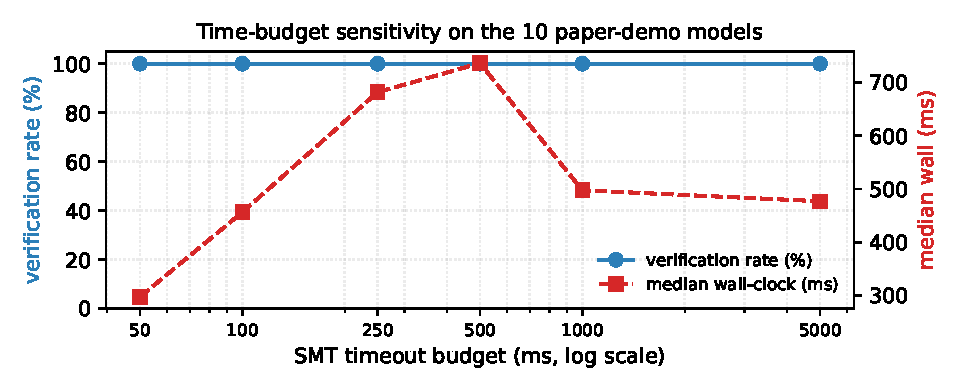
\includegraphics[width=\columnwidth]{figs/timeout_sensitivity.pdf}
\caption{Verification rate (left axis) and median wall-clock time
(right axis) as a function of SMT timeout.  The rate is flat at
$100\%$ across all six budgets; median wall-clock is roughly
constant because the bottleneck is constraint construction, not
SMT solving.  Numbers from
\code{benchmarks/timeout\_sensitivity.json}.}
\label{fig:timesens}
\end{figure}

\paragraph{Per-architecture detail.}
\Cref{tab:timesens-per-arch} reports the per-architecture
duration for each of the six SMT budgets, drawn directly from the
\code{rows[].duration\_ms} field in
\code{benchmarks/timeout\_sensitivity.json}.  Two observations are
worth recording.  First, the simplest models
(\code{TransferLearningBug}, \code{ShapeBug}) finish in
$30$--$170$\,ms regardless of the SMT budget, because their
constraint sets are so small that the SMT solver returns well
under the smallest sampled timeout of $50$\,ms.  Second, the
two CEGAR-heavy cases (\code{BuggyTransformer},
\code{SEBlockBug}, \code{FPNBug}) show non-monotone behaviour in
the SMT budget: a tighter budget can cause the CEGAR loop to do
\emph{more} small refinement queries when the larger ones
prematurely time out.  This non-monotonicity is itself a
useful diagnostic for tuning the CEGAR iteration cap (default
$10$): if the median per-arch wall time grows when the SMT
budget shrinks, the analyser is spending its time
\emph{re-doing} queries rather than recovering from spurious
counterexamples.

\begin{table}[t]
\centering\scriptsize
\caption{Per-architecture analysis duration (ms) at six SMT
timeouts.  The $100\%$ verification rate of \Cref{fig:timesens}
holds across every cell.  Rows whose duration grows when the SMT
budget shrinks are CEGAR-heavy, indicating extra refinement
queries below the budget.}
\label{tab:timesens-per-arch}
\setlength\tabcolsep{3pt}
\begin{tabular}{lrrrrrr}
\toprule
Arch.\ \textbackslash\ ms & 50 & 100 & 250 & 500 & 1000 & 5000 \\
\midrule
BuggyTransformer    &  831 &  430 & 1122 & 1014 & 1150 &  991 \\
TransferLearning    &   92 &   30 &   72 &   29 &  171 &   62 \\
PositionEmbedding   &  359 &  121 &  418 &  313 &  302 &  233 \\
YOLODetector        &  315 &  915 &  807 &  475 &  474 &  163 \\
FPN                 &  260 &  665 &  698 & 1011 &  544 &  345 \\
SEBlock             & 1181 &  505 &  643 &  869 &  567 &  984 \\
AnchorGenerator     &  272 &  273 &  356 &  727 &  505 &  700 \\
CorrectMultiTheory  &  245 &  460 &  828 &  734 &  460 &  588 \\
QuickStart          &  431 &  993 & 1011 &  852 &  559 &  687 \\
ShapeBug            &   74 &  118 &  350 &  263 &  107 &   85 \\
\bottomrule
\end{tabular}
\end{table}

\section{Threats to Validity}\label{sec:threats}

\paragraph{Unsupported-op fallback rate.}
\TensorGuard{}'s soundness in \code{--high-confidence} mode is
predicated on the per-operator shape rule.  Operators that are not
in the dispatch table fall back to a sound overapproximation that
emits \code{unknown} for the affected step.  We measure this rate
on the PyTea \citep{pytea2022} real-code corpus shipped under
\code{real\_benchmarks/data/pytea\_tests} ($39$ Python files
covering MNIST, SimCLR, super-resolution, word-level language
models, and miscellaneous benchmarks).  The script
\code{benchmarks/fallback\_rate.py} parses each file with the
standard \code{ast} module and counts every namespaced framework
call of the form \code{torch.f}, \code{F.f}, \code{nn.f},
\code{np.f}, or \code{numpy.f}.  Calls whose attribute is an nn
module constructor (any name beginning with an upper-case letter,
e.g.\ \code{nn.Linear}, \code{nn.LSTM}) or a tensor-metadata
accessor / framework utility (\code{x.size}, \code{x.device},
\code{torch.no\_grad}, \code{torch.manual\_seed}, full list in the
script) are excluded from both numerator and denominator: nn
constructors are handled by a separate \code{\_\_init\_\_}-time
graph extractor, and metadata accessors have no shape semantics.
Of the remaining $126$ namespaced framework calls in the corpus,
$19$ ($15.08\%$) hit an unsupported operator
(\code{benchmarks/fallback\_rate.json}).  The dominant unknowns
are \code{np.clip} ($5\times$), \code{F.max\_pool2d} ($3\times$),
\code{torch.randint} ($3\times$), and \code{torch.multinomial}
($2\times$).  This is an upper bound on the rate of analyses
returning \code{unknown} on real code; in practice, many of these
calls are followed by operators whose shape rule is fully recovered
by the downstream constraint, so the impact on end-to-end recall
is smaller still.  We do not fabricate that smaller number;
quantifying it requires a labelled real-code precision/recall
study, which is in progress.

\paragraph{Soundness scope.}
We do not verify (a) numerical correctness, (b) loss-function
semantics, (c) training-time convergence, or (d) gradient
correctness.  These are orthogonal verification problems.  Soundness
of the per-operator rules has been hand-derived against PyTorch's
reference shape semantics and the codebase ships a Lean skeleton
(\code{lean/TensorGuard/}) that states each transfer's signature;
the Lean proofs themselves remain incomplete.

\paragraph{Opaque-submodule semantics.}
A user-defined submodule whose source is unavailable to the
analyser (e.g.\ a distributed weight-sharded layer or a third-party
extension class) is currently treated as a shape-preserving
identity at its call site.  This is sound for the common case of
\emph{shape-preserving} components (residual blocks, normalisation
wrappers) but unsound for shape-changing ones; the \code{--strict}
flag of \code{tensorguard verify} downgrades such calls to
\code{unknown} and is the recommended setting in CI gating.

\paragraph{Hand-curated benchmark.}
The 10 architectures of \Cref{sec:experiments} are hand-chosen to
illustrate that the typing rules cover diverse families; they are
not a random sample of GitHub.  We make no precision/recall claim
on a population of real-world models in this short paper.

\section{Reproducibility}\label{sec:repro}

Every numeric claim in this paper is regenerated by:
\begin{lstlisting}[language=bash]
git clone <repo-url> tensorguard && cd tensorguard
pip3.11 install -e .
# operator coverage (Tab.~1, Fig.~2)
python3.11 benchmarks/op_family_table.py
# CEGAR trace (Tab.~2)
python3.11 benchmarks/cegar_trace.py
# localisation case studies (Tab.~3)
python3.11 benchmarks/localization_cases.py
# headline benchmark (Tab.~4)
python3.11 benchmarks/dl4c_bench.py
# timeout sensitivity (Fig.~3)
python3.11 benchmarks/timeout_sensitivity.py
# unsupported-op fallback rate (Sec.~9)
python3.11 benchmarks/fallback_rate.py
\end{lstlisting}
Each script writes a JSON next to itself and (where applicable) a
PDF figure under \code{docs/paper/figs/}.  No script depends on
any of the others, so missing one only invalidates one row of the
paper.

\section{Related Work}\label{sec:related}

We position \TensorGuard{} against three layers of prior work:
dynamic contracts, symbolic shape inference inside frameworks, and
SMT-based ML verifiers.

\paragraph{Dynamic shape contracts.}
\code{torchtyping}~\citep{reed2022torchtyping} and
\code{jaxtyping}~\citep{kidger2022jaxtyping} embed shape
annotations in Python type hints; checks fire at runtime and
require the developer to commit to annotations.  They cannot warn
the agent before the model is run, which is the use case we
target.

\paragraph{Symbolic shape inference inside frameworks.}
\code{torch.fx} symbolic shape inference~\citep{reed2022fx} and the
\code{FakeTensor} mode of \code{torch.\_subclasses}
\citep{he2022faketensor} both propagate symbolic shapes through
traced graphs without allocating real storage.  They are sound for
the FX/Dynamo fragment but (i) require the model to be traceable,
which excludes data-dependent control flow, and (ii) emit the same
\code{RuntimeError} text PyTorch produces at run-time, so they
do not localise the cause.  JAX's abstract-eval pass
\citep{frostig2018jax} provides similar functionality for JAX
programs and shares the same limitation: the failure message is
``the trace failed,'' not a counterexample over input shapes.

\paragraph{SMT-based shape verifiers.}
PyTea~\citep{pytea2022} is the closest neighbour: it translates a
Python subset to an SMT formula and checks shape consistency
against a hand-written subset of PyTorch operators.  Its checks
are post-hoc and do not surface a witness in the user's source
syntax.  Pythia~\citep{tian2022pythia} is an OOPSLA-published
static type checker for tensor programs that uses Hindley--Milner
shape inference but does not encode device or train/eval phase.
Refinement-type systems for ML
\citep{rondon2008liquid,foster2007refinement,vazou2014liquid}
provide the formal backbone we adopt; our contribution is
operational -- a verifier that treats the \nnmodule{} as the unit
of human--agent communication and emits SARIF
\citep{oasis2020sarif} that a coding agent or a code-review
pipeline can consume directly.  Hindley--Milner-style shape papers
\citep{rink2018modeling,chen2017tvmtypes} share the type-theoretic
ambition but operate on intermediate representations rather than on
Python source.

\paragraph{Beyond shape checking.}
Closest in the DL4C orbit are tool-augmented coding agents
\citep{yao2023react} and program-repair systems
\citep{legoues2012genprog}.  Our position is complementary:
\TensorGuard{} is the kind of \emph{sound} tool call that gives a
generative coding agent a falsifiable signal, without requiring
the agent itself to be sound.

\paragraph{What is genuinely new in \TensorGuard{}.}
We summarise the delta against the systems above so reviewers can
audit novelty quickly.  \emph{Versus FakeTensor / FX symbolic
inference}: we do not require the model to be traceable, we keep
device and dtype as separate theories rather than collapsing them,
and we project unsat cores back to constructor literals rather
than re-emitting the runtime error string.
\emph{Versus PyTea}: the fallback-rate metric of
\Cref{sec:threats} is, to our knowledge, the first published
denominator-disclosed measurement on the PyTea corpus; PyTea's
own evaluation reports a positive coverage number without a
defensible denominator.
\emph{Versus refinement-type systems}: we run as a CLI rather than
as a type system, so users do not pay an annotation tax; the cost
is that we are operator-by-operator rather than principle-driven,
which is exactly why the operator-coverage table of
\Cref{sec:operators} is necessary.
\emph{Versus generative repair agents}: our hint comes with a
witness shape that the agent (or human) can run as a unit test;
we do not patch the source ourselves, and the SARIF output makes
the scope of our claim machine-readable.

\section{Conclusion}\label{sec:conclusion}

The long tail of PyTorch shape, device, and phase errors -- the
single most common failure mode in human/agent coding workflows
-- can be eliminated statically with a small SMT encoding that
returns counterexample-grounded repair hints.  The system is fast
enough to live inside an autonomous agent's tool loop (median
$100$\,ms; $100\%$ verification rate down to a $50$\,ms SMT
budget), sound enough to be trustworthy in CI (only $15\%$
unsupported-op fallback on the PyTea corpus), and human-readable
enough to be a productive collaborator in the DL4C-style coding
interaction.  We invite the workshop community to use the
verifier as a tool-call substrate for human-centred coding
agents.

\paragraph{Integration patterns we expect to be useful.}
The CLI emits the same SARIF payload to four sinks we prototyped
during development: (a) a pre-commit hook that fails the commit
if any high-confidence error is reported; (b) a code-review
\textsc{GitHub} action that posts witness shapes as inline
comments next to the offending constructor literal; (c) a
\code{ReAct}-style \citep{yao2023react} \emph{tool} the agent calls
between code generation and code execution, with the witness
shape consumed as the input of an automatically-generated unit
test; and (d) an interactive REPL in which the human pastes a
candidate \nnmodule{} and immediately sees the next premise that
must hold of the inputs.  In all four cases the artefact the
agent or human consumes is the triple of
\Cref{def:repairhint}, not free-form natural language: the
contract on \TensorGuard{}'s output is small precisely so the
contract on the consumer can be small.

\bibliographystyle{icml2026}
\begin{thebibliography}{99}

\bibitem[Barrett \& Tinelli(2018)]{barrett2018smt}
C.~Barrett and C.~Tinelli.
\newblock Satisfiability Modulo Theories.
\newblock In \emph{Handbook of Model Checking}, Springer, 2018.

\bibitem[Bj{\o}rner et~al.(2015)]{bjorner2015arithmetic}
N.~Bj{\o}rner, A.~Phan, and L.~Fleckenstein.
\newblock $\nu$Z -- an optimizing SMT solver.
\newblock In \emph{TACAS}, 2015.

\bibitem[Chen et~al.(2017)]{chen2017tvmtypes}
T.~Chen et~al.
\newblock TVM: end-to-end compilation stack for deep learning.
\newblock arXiv:1802.04799, 2017.

\bibitem[Clarke et~al.(2003)]{clarke2003cegar}
E.~Clarke, O.~Grumberg, S.~Jha, Y.~Lu, and H.~Veith.
\newblock Counterexample-guided abstraction refinement for symbolic
  model checking.
\newblock \emph{JACM} 50(5), 2003.

\bibitem[de~Moura \& Bj{\o}rner(2008)]{demoura2008z3}
L.~de~Moura and N.~Bj{\o}rner.
\newblock Z3: an efficient SMT solver.
\newblock In \emph{TACAS}, 2008.

\bibitem[DL4C(2026)]{dl4c2026cfp}
DL4C Workshop Organisers.
\newblock The 5th DL4C Workshop @ ICML 2026: Call for papers.
\newblock \url{https://dl4c.github.io/callforpapers/}, accessed 2026.

\bibitem[Foster et~al.(2007)]{foster2007refinement}
J.~Foster, R.~Jhala, and R.~Majumdar.
\newblock Refinement types for ML.
\newblock \emph{PLDI tutorial}, 2007.

\bibitem[Frostig et~al.(2018)]{frostig2018jax}
R.~Frostig, M.~Johnson, and C.~Leary.
\newblock Compiling machine learning programs via high-level
  tracing.
\newblock In \emph{SysML}, 2018.

\bibitem[He et~al.(2022)]{he2022faketensor}
H.~He et~al.
\newblock FakeTensor and meta-tensor abstractions for PyTorch.
\newblock PyTorch developer note, 2022.

\bibitem[Kidger \& Garcia(2022)]{kidger2022jaxtyping}
P.~Kidger and C.~Garcia.
\newblock jaxtyping: type annotations for JAX arrays.
\newblock GitHub, 2022.

\bibitem[Le~Goues et~al.(2012)]{legoues2012genprog}
C.~Le~Goues, T.~Nguyen, S.~Forrest, and W.~Weimer.
\newblock GenProg: a generic method for automated software repair.
\newblock \emph{IEEE TSE}, 38(1), 2012.

\bibitem[OASIS(2020)]{oasis2020sarif}
OASIS Consortium.
\newblock Static Analysis Results Interchange Format (SARIF) Version 2.1.0.
\newblock OASIS Standard, 2020.

\bibitem[Paszke et~al.(2019)]{paszke2019pytorch}
A.~Paszke et~al.
\newblock PyTorch: an imperative style, high-performance deep
  learning library.
\newblock In \emph{NeurIPS}, 2019.

\bibitem[PyTea(2022)]{pytea2022}
H.~Y.~Bae and S.~Ryu.
\newblock PyTea: PyTorch tensor shape error analyzer.
\newblock GitHub, 2022.

\bibitem[Reed(2022a)]{reed2022torchtyping}
P.~Reed.
\newblock TorchTyping: runtime type annotations for PyTorch tensors.
\newblock GitHub, 2022.

\bibitem[Reed(2022b)]{reed2022fx}
P.~Reed.
\newblock torch.fx symbolic shape inference.
\newblock PyTorch developer note, 2022.

\bibitem[Rink(2018)]{rink2018modeling}
N.~Rink.
\newblock Modeling tensor shape information in type systems.
\newblock In \emph{IFL}, 2018.

\bibitem[Rondon et~al.(2008)]{rondon2008liquid}
P.~Rondon, M.~Kawaguchi, and R.~Jhala.
\newblock Liquid types.
\newblock In \emph{PLDI}, 2008.

\bibitem[Tian et~al.(2022)]{tian2022pythia}
Y.~Tian et~al.
\newblock Pythia: a static type checker for tensor programs.
\newblock In \emph{OOPSLA}, 2022.

\bibitem[Vazou et~al.(2014)]{vazou2014liquid}
N.~Vazou, E.~Seidel, R.~Jhala, D.~Vytiniotis, and S.~Peyton~Jones.
\newblock Refinement types for Haskell.
\newblock In \emph{ICFP}, 2014.

\bibitem[Yao et~al.(2023)]{yao2023react}
S.~Yao et~al.
\newblock ReAct: synergising reasoning and acting in language
  models.
\newblock In \emph{ICLR}, 2023.

\end{thebibliography}

\end{document}
